\section{Conclusion}

\begin{frame}{Class Summary}
  In this class we saw several algorithms for calculating computational geometry constructs:\bigskip

  \begin{itemize}
    \item Points and Lines and Intersections;
    \item Circles and Triangles, areas and intersections;
    \item Convex Hull testing and Convex Hull construction;
  \end{itemize}\bigskip

  Harder geometry problems will require you to perform search on geometry constructs, graph search, etc. Having a library with the functions of this class ready will be useful!
\end{frame}

\subsection{Problem Discussion}
\begin{frame}
  \frametitle{This Week's Problems}
  \begin{itemize}
    \item Sunny Mountains -- Line and Points
    \item Waterfall -- Line and Points\\{\bf Discussed in Class}
    \item Elevator -- Circles and Rectangles
    \item Colorful Flowers -- Circles and Triangles
    \item Bounding Box -- Circles, Triangles and Polygons\\{\bf Discussed in Class}
    \item Soya Milk -- Rectangle and Triangle\\{\bf Discussed in Class}
    \item Trash Removal -- Polygon Manipulation
    \item Board Wrapping -- Convex Hull
  \end{itemize}
\end{frame}

\begin{frame}{Sunny Mountains}
  \begin{center}
    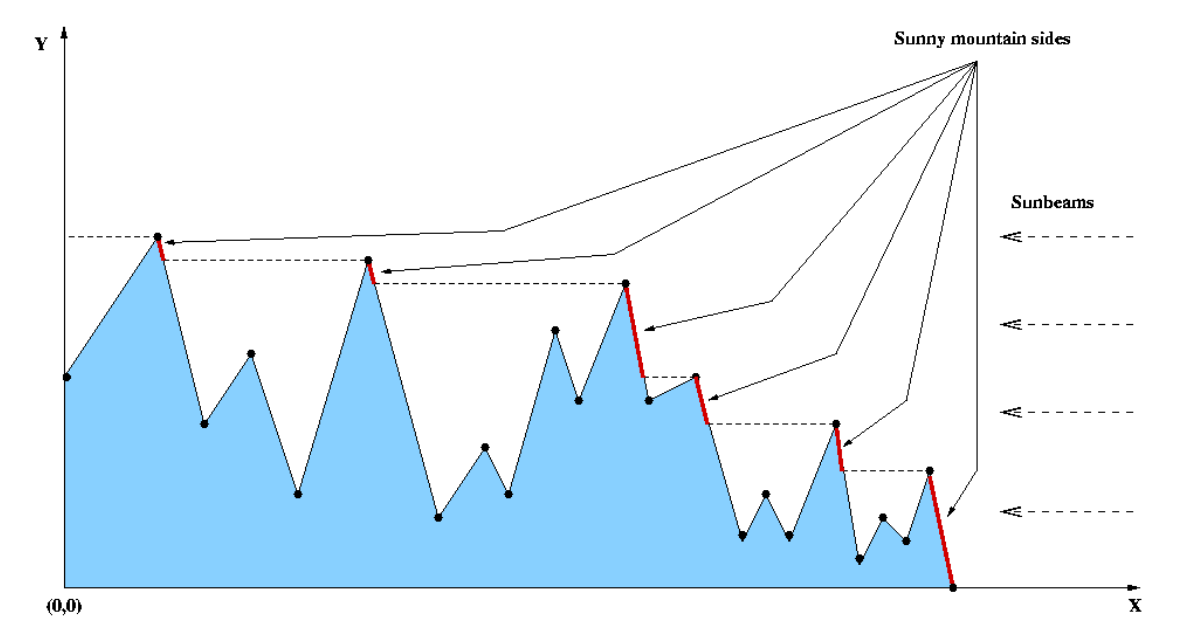
\includegraphics[width=.7\textwidth]{../img/problem_sunnyside}
  \end{center}
  \begin{itemize}
    \item Given segment points as the input, calculate the area illuminated by the sun.\bigskip

    \item {\bf Hint:} This problem is about calculating line/segment intersections.
    \item {\bf Hint:} Because the line is always HORIZONTAL, you can write a function that is simpler than the one I introduced in this class.
  \end{itemize}
\end{frame}

\begin{frame}{Elevator}
  \begin{center}
    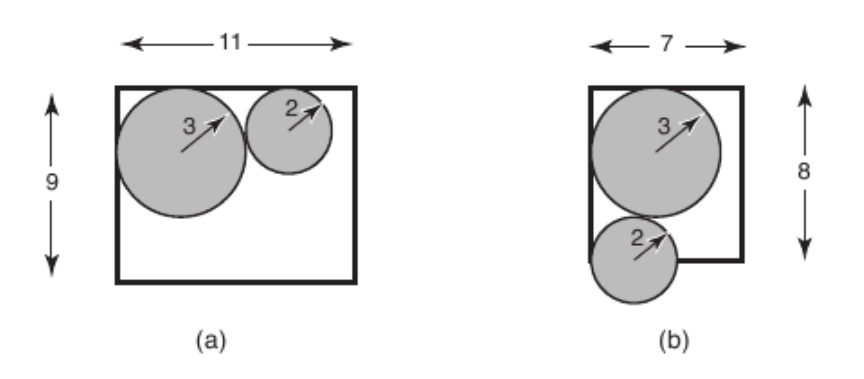
\includegraphics[width=.7\textwidth]{../img/problem_elevator}
  \end{center}
  \begin{itemize}
    \item {\bf Input:} Size of the elevator and two Radius: $R_1$, $R_2$.
    \item {\bf Output:} Do the two circles fit in the elevator? Y/N?
    \item {\bf Hint:} The code is very simple, solve this program on paper first.
  \end{itemize}
\end{frame}

\begin{frame}{Colorful Flowers}
  \begin{center}
    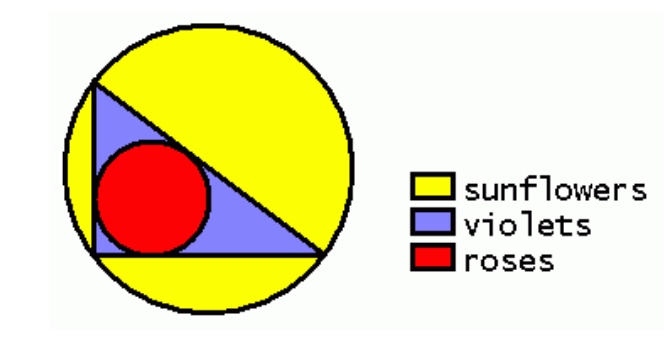
\includegraphics[width=.5\textwidth]{../img/problem_colourful}
  \end{center}
  \begin{itemize}
    \item {\bf Input}: Three sides of blue triangle
    \item {\bf Output}: Area of Yellow Zone, Blue Zone and Red Zone
    \item {\bf Hint}: Practice the code for incircle and circumcircle!
  \end{itemize}
\end{frame}

\begin{frame}{Trash Removal}
  \begin{center}
    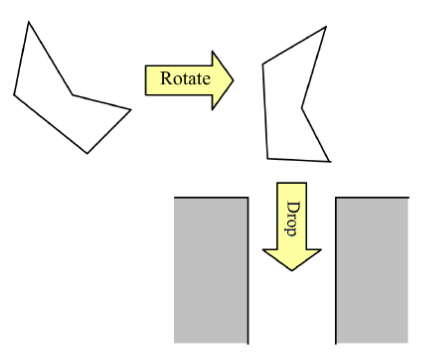
\includegraphics[width=.5\textwidth]{../img/problem_trash}
  \end{center}
  \begin{itemize}
    \item What is the smallest trash box that can fit the polygon (trash)
    \item {\bf Input}: Vertices of the polygon
    \item {\bf Output}: Size of the smallest trash that fits the polygon
    \item {\bf Hint}: It might help to think of the convex version of the polygon
  \end{itemize}
\end{frame}

\begin{frame}{Board Wrapping}
  \begin{center}
    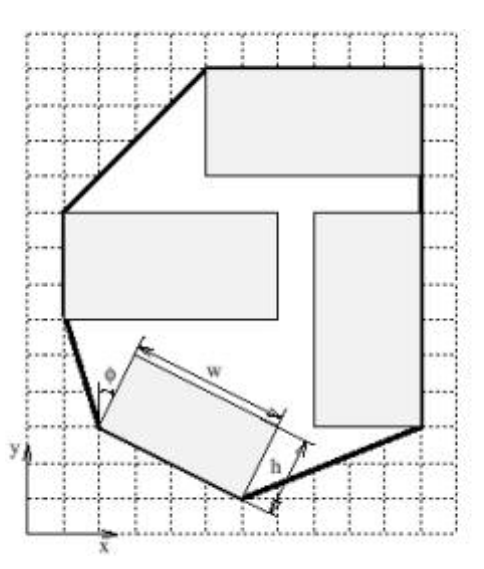
\includegraphics[width=.4\textwidth]{../img/problem_wrapping}
  \end{center}
  \begin{itemize}
    \item Convex Hull problem;
    \item Don't forget to rotate the rectangles correctly during input!
  \end{itemize}
\end{frame}
